
%(BEGIN_QUESTION)
% Copyright 2010, Tony R. Kuphaldt, released under the Creative Commons Attribution License (v 1.0)
% This means you may do almost anything with this work of mine, so long as you give me proper credit

This distillation tower separates a mixed ``feed'' liquid into two different products called ``distillate'' and ``bottoms'', using a liquid flow control loop to regulate feed coming into the middle of the tower:

$$\includegraphics[width=15.5cm]{i03690x01.eps}$$

Suppose an instrument technician mis-calibrates the feed flow transmitter so that it outputs less signal than it should (representing less liquid flow than is actually going into the tower).  What effect will this have on the actual liquid flow rate to the tower?  Will the actual liquid flow rate become {\it less} than it should be, {\it more} than it should be, or will it remain exactly {\it as} it should be?

\underbar{file i03690}
%(END_QUESTION)





%(BEGIN_ANSWER)

The actual feed flow rate will be {\bf greater} than it should be as a result of the fault.

%(END_ANSWER)





%(BEGIN_NOTES)

{\bf This question is intended for exams only and not worksheets!}.

%(END_NOTES)


